\subsection{Minimal Materialization Plan Enumeration}
\label{ssec:enumeration}

\begin{algorithm}[t]
   \caption{Enumerate valid minimal materialization plans.} 
   \label{alg:enumerate}
   \footnotesize
   \begin{algorithmic}[1]
      \Statex \textbf{Input}: a set of rules R.
      \Statex \textbf{Output}: a set of valid minimal view materialization plans.
      \State G $\gets ~ \text{constructReplacementGraph}(R)$
      \State B $\gets ~ \text{getMinimal}(\text{getBaseSet}(R))$
      \State Q $\gets ~ \{ B \}$
      \State minPlans $\gets ~ \{ B \}$
      \While {$Q \neq \emptyset$}
        \State V $\gets$ Q.pop()
        \State nextPlans $\gets ~ \{ \text{getMinimal(p)} ~|~ p \in \text{replace}(V,G) \}$
        \State minPlans $\gets$ minPlans $\cup$ nextPlans
        \State Q $\gets$ Q $\cup$ \text{nextPlans}
      \EndWhile
      \State \Return minPlans

    \vspace{2mm}

    \Function{constructReplacementGraph}{R}
            \State $G \gets \emptyset$
            \For{each relation $r$ in R}
                \State $ P \gets \text{definingRules}(r,R) $
                \If{$P$ contains no aggregation, transaction rule}
                    \State $U \gets \{ \bigcup_{p \in P} p.body.relation \}$
                    \If{$U$ contains no transaction relations}
                        \State $G \gets G \cup \{(u, r) | u \in U \} $
                    \EndIf
                \EndIf
            \EndFor
            \State \Return G
    \EndFunction

    \vspace{2mm}


    \Function{getMinimal}{V}
            \State $M \gets V$
            \For{each relation $v$ in V}
                \State $M' \gets M \setminus \{ v \}$
                \If{isValid($M'$)}
                    \State $M \gets M'$
                \EndIf
            \EndFor
            \State \Return M
    \EndFunction

    \vspace{2mm}

    \Function{replace}{V,G}
            \State replacements $\gets \emptyset$
            \For{v in V}
                \State $U \gets \{ u | (u,v) \in G \}$
                \State newPlan $\gets V \setminus \{ v \} \cup U$
                \State replacements $\gets $ replacements $\cup \{ \text{newPlan}\} $
            \EndFor
            \State \Return replacements
    \EndFunction
      
   \end{algorithmic}
\end{algorithm}


Generating materialization plans is outlined in Algorithm~\ref{alg:enumerate}. 
Initially, the algorithm creates a supplementary data structure known as the replacement graph $G$. 
This graph is built based on the dependency information obtained from the set of rules $R$. 
The construction of the graph is explained in 
{\sf ConstructReplacementGraph} function (lines 11-19).

\noindent \textbf{Base minimal materialization plan.}
Algorithm~\ref{alg:enumerate} starts with generating a base valid materialization plan composed of relations necessarily to be fetched by the optimized imperative control flow. This base plan represents the read-only approach: storing all relations that could be accessed during transaction execution or public queries, without any on-demand computation. The base materialization plan is then reduced to the minimal form (Definition~\ref{def:min-plan}), based on the {\sf getMinimal} function (lines 20-26), which will be discussed later.

For instance, the base materialization plan for the example contract in Figure~\ref{fig-example} initially includes relations {\sf “totalSupply”}, {\sf “balanceOf”}, {\sf “permission”}, and {\sf “canSend”}. This is because, through arithmetic optimization in Sec~\ref{ssec:arith_view}, view relations such as {\sf “totalMint”}, {\sf “totalBurn”}, {\sf “totalIn”}, and {\sf “totalOut”} are simplified from the control flow and therefore not included in the base plan. Similarly, transaction records like {\sf “mint”}, {\sf “burn”}, and {\sf “transfer”}, which are incrementally inserted in response to each incoming transaction and not revisited later, are also omitted from the base plan. Then we derive the minimal form of this base plan, which consists of {\sf “totalSupply”}, {\sf “balanceOf”}, {\sf “permission”}, as {\sf “canSend”} can be derived given the executability of {\sf “permission”}. Note that we could not remove {\sf “permission”} but keep {\sf “canSend”} since this will lose excutability for relation {\sf “permission”} itself.


\noindent \textbf{Construct replacement graph.}
The {\sf ConstructReplacementGraph} function showcases the process of constructing the replacement graph. 
Given a set of rules $R$ in a \base program. For each relation $r$ in $R$, it initially identifies the set of defining rules (Definition~\ref{def:defining-rules}) of $r$, denoted as P (line 14). 
If $P$ contains aggregation rules or transaction rules, then using the pruning patterns discussed in Section~\ref{ssec_pruning}, relation $r$ will not be considered for on-demand computation, and hence, no corresponding replacement information will be added to the replacement graph $G$.

For example, consider the following rule that defines the relation {\sf "totalSupply"} (Figure ~\ref{fig-example}, line 17):
\[ \texttt{totalSupply(s)}:-\texttt{totalMint(m)}, \texttt{totalBurnt(b)}, s:=m-b \]
It defines {\sf totalSupply} as the difference between the sum of the minted amount ({\sf totalMint}) 
and the sum of the burnt amount ({\sf totalBurn}). 
Based on this rule, two edges are added to the replacement graph: 
({\sf \lstinline{totalMint}, \lstinline{totalSupply}}) and ({\sf \lstinline{totalBurn}, \lstinline{totalSupply}}). 
Consequently, it is possible to choose not to materialize {\sf totalSupply} but instead materialize {\sf totalMint} and {\sf totalBurn} relations. 
When queried, the value of {\sf totalSupply} can be computed from these two materialized relations. 
This replacement choice reflects the beneficial dynamic exploration of our view selection algorithm: 
Though the optimized control flow requires only the executability of {\sf totalSupply} rather than the executability of {\sf totalMint} and {\sf totalBurn} which could be simplified by view elimination, 
{\sf totalMint} and {\sf totalBurn} can still be chosen to be materialized and executable to support the executability of {\sf totalSupply}  by lazy evaluation if {\sf totalSupply} itself is not materialized.

If we delve deeper into the definition of {\sf totalMint} on Figure~\ref{fig-example} line 15, we observe that it is defined as a sum over the {\sf "mint"} transaction relation on the second column, which represents the transaction amount. 
However, calculating {\sf totalMint} on demand is not feasible 
since it would require iterating over all {\sf mint} transaction records to obtain the sum. 
Consequently, no replacement edges are added to the replacement graph for relations defined on aggregation rules. 
Besides, by rule 4 in Section~\ref{ssec_pruning}, transaction relations defined by transactions rules as Figure~\ref{fig-example} line 2-7
are not considered for replacement (Algorithm~\ref{alg:enumerate}, lines 15 to 18).

Otherwise, it is feasible to materialize all the relations in $r$'s defining rules and realize relational queries to $r$ whenever necessary. Consequently, for each $r$'s defining relation $u$ in $U$, an edge is included from $u$ to $r$ to signify that on-demand recomputation of relation $r$ requires information of relation $u$. Figure~\ref{fig:replacement-graph} shows the replacement graph constructed from the example contract in Figure ~\ref{fig-example}.

\begin{figure}[ht]
    \centering
    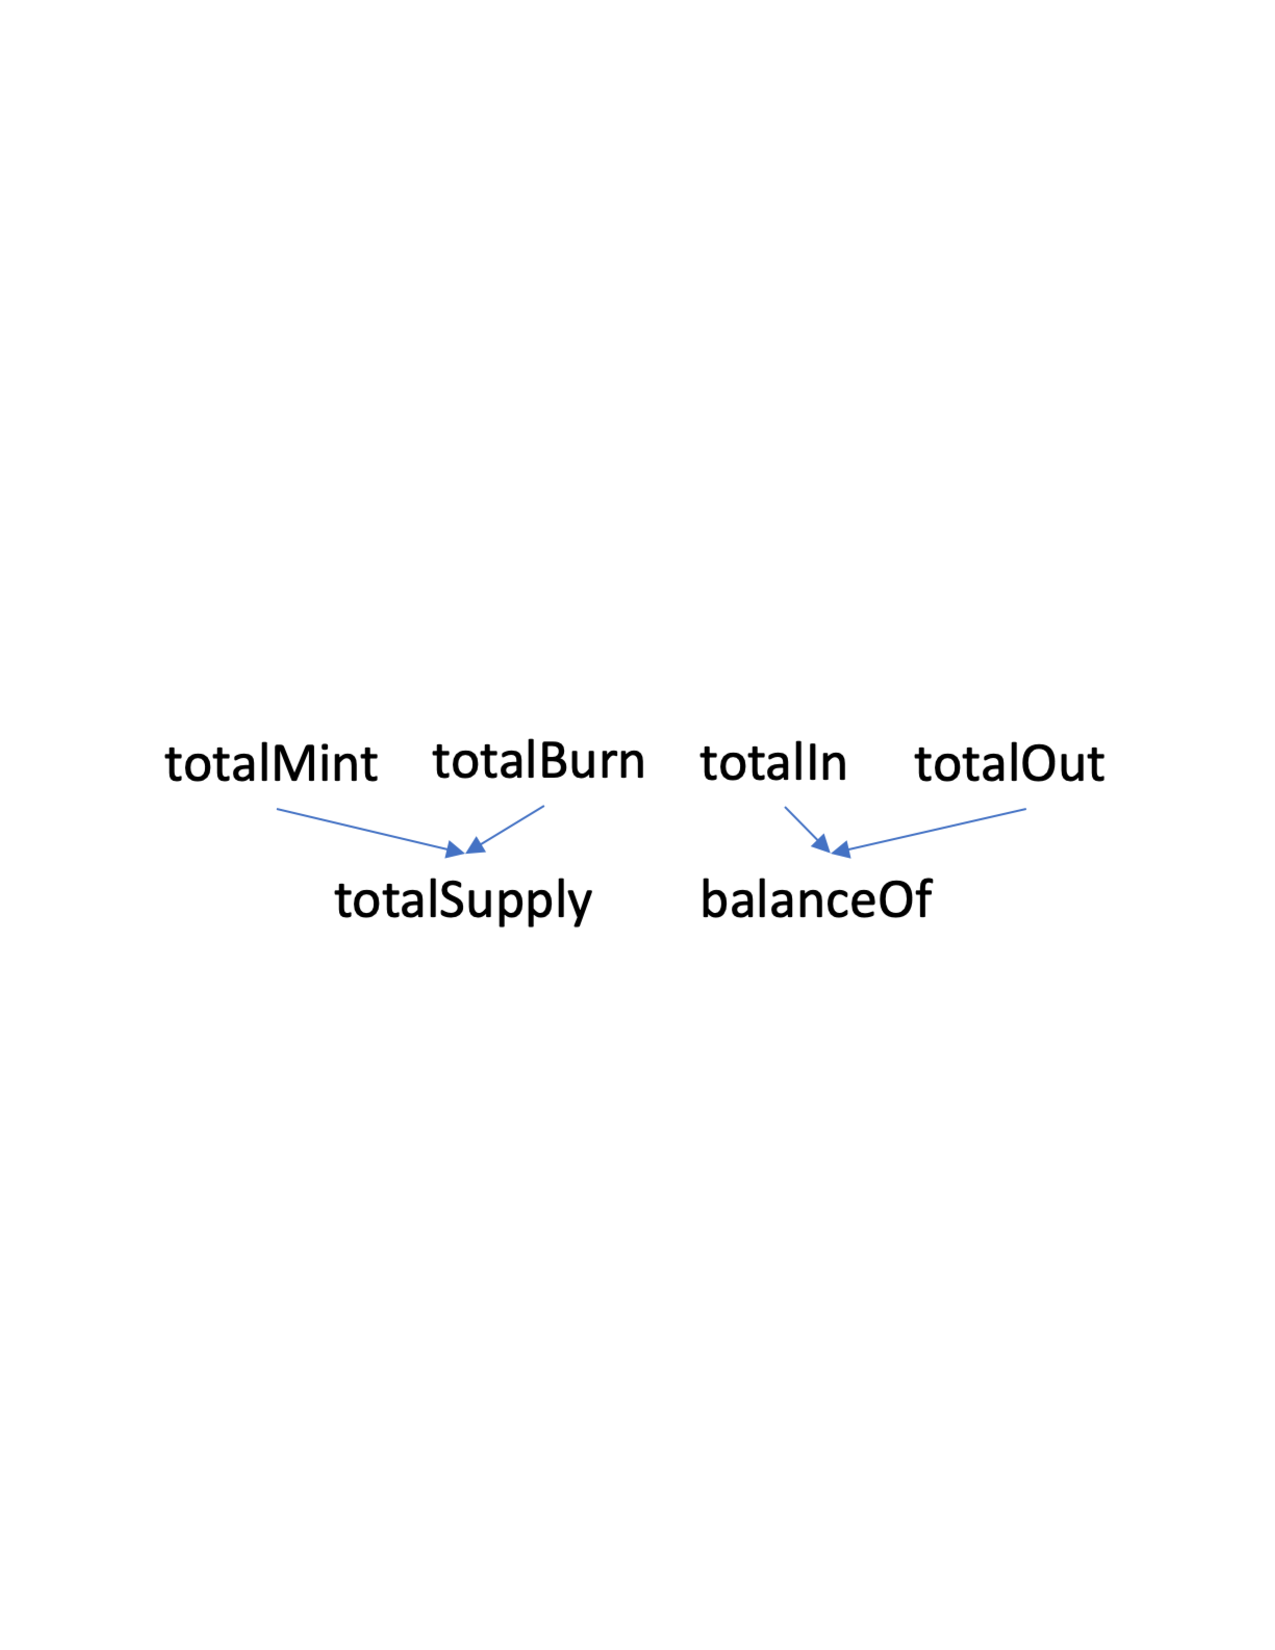
\includegraphics[width=0.3\textwidth]{figures/replacement-graph.pdf}
    \caption{Replacement graph of example contract}
    \label{fig:replacement-graph}
\end{figure}


% \begin{algorithm}[t]
%     \caption{Generate valid alternative plans.}
%     \label{alg:replace}
%     \footnotesize
%     \begin{algorithmic}[1]
%         \Statex \textbf{Input}: a valid materialization plan $V$, 
%            a replacement graph G. 
%         \Statex \textbf{Output}: a set of all valid alternative plans for $V$.  
%         \Function{replace}{V,G}
%             \State replacements $\gets \emptyset$
%             \For{v in V}
%                 \State $U \gets \{ u | (u,v) \in G \}$
%                 \State newPlan $\gets V \setminus \{ v \} \cup U$
%                 \State replacements $\gets $ replacements $\cup \{ \text{newPlan}\} $
%             \EndFor
%             \State \Return replacements
%         \EndFunction
%     \end{algorithmic}
% \end{algorithm}

\noindent \textbf{Minimize materialization plans.}
The goal of this step is to remove redundant relations,
which could be introduced during base plan construction and relation replacement.
A relation is redundant if it can be removed without impacting the validity of the materialization plan.
The {\sf getMinimal} function (lines 20-26) shows the minimization step.
Given a view materialization plan $V$, for each relation $v$ in $V$, it checks whether removing $v$ affects the validity of the resulting materialization plan $M'$. If $M'$ is valid, $v$ is removed from the minimal form. Otherwise, $v$ is kept in the minimal form. A beneficial feature of our algorithm when starting at the base minimal plan is that the later generated plan will converge to its unique minimal form, regardless of the order of removing relations.
A proof of the uniqueness property is presented in Section~\ref{sec-proof}.

\noindent \textbf{Generate alternative materialization plans via replacement.} 
The {\sf replace} function (algorithm~\ref{alg:enumerate}, lines 27-33) presents the generation of alternative view materialization plans. It takes a valid materialization plan $V$ and a replacement graph $G$ as input. For each relation $v$ in $V$, it queries $G$ for incoming edges and puts the vertices on all incoming edges into a set $U$. It then generates an alternative materialization plan by replacing $v$ with the set of relations in $U$. For example, given the replacement graph shown in Figure~\ref{fig:replacement-graph} and a materialization plan $V$ that includes {\sf totalSupply} relation, it would replace {\sf totalSupply} with {\sf totalMint} and {\sf totalBurn} relations as a new materialization plan. The algorithm iterates over all the relations in $V$ and returns the set of all newly discovered materialization plans.

\noindent \textbf{Overall algorithm.} 
Overall, algorithm~\ref{alg:enumerate} enumerates all valid minimal materialization plans in a breadth-first search fashion. 
A queue $Q$ is used to store all the plans to be explored for alternatives, and is initialized by the minimal base materialization plan.
Starting from the initial choice, it iteratively generates alternative choices for each plan through relation replacements based on the replacement graph $G$. 
The set of generated alternative replacement plans is also turned into their minimal forms, and then added to the queue $Q$ and the collection $minPlans$. 
This iterative process continues until the queue is empty, at which point the algorithm returns $minPlans$ as the final solution.